\begin{figure}[H]
  \centering
  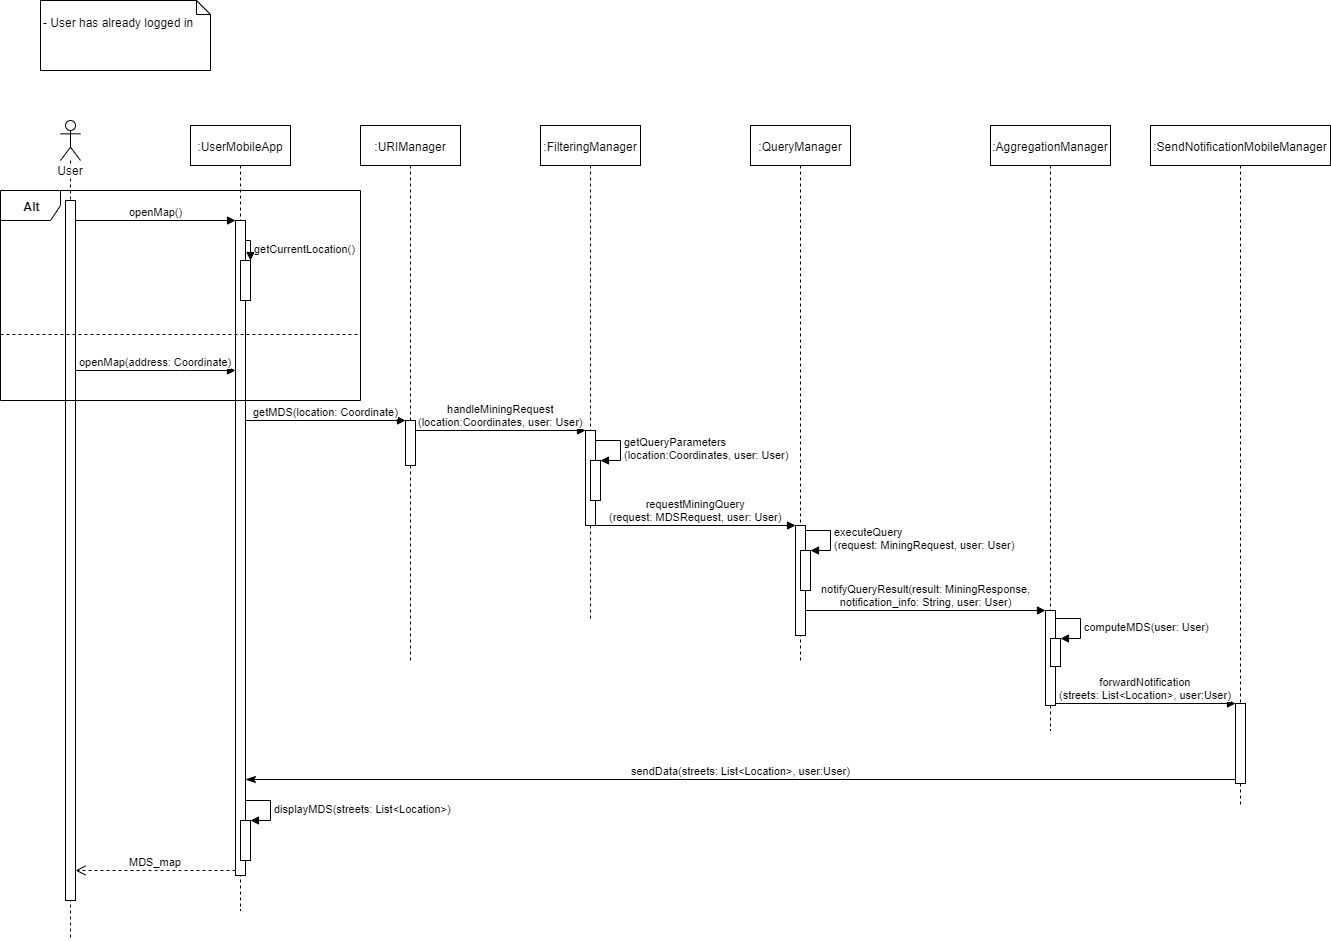
\includegraphics[width=1\textwidth]{Images/UML_diagrams/Sequence_Diagrams/Request_MDS_sd.png}
  \caption{Watch Most Dangerous Streets sequence diagram}
  \label{fig:watch_MDS_sd}
\end{figure}
This sequence diagram represents the second main functionality of the user application, that is to say the visualization of the most dangerous streets. As soon as the user taps on the map section of the mobile application, a request for the MDS streets is sent to the URIManager. By default the MDS are requested in an area nearby the current location of the user, but if the user wishes to ask for the MDS around a specific location he can insert the address in the search bar and then the request will be based on that coordinates; once the request is complete it is forwarded to the FilteringManager via the URIManager. When the FilteringManager receives the request, it will automatically collect the query parameters that are necessary for that operation.  Once all the parameters are collected, the FilteringManager sends a MiningRequest to the QueryManager that will execute a query based on those parameters. As soon as the execution of the query is finished the output data is sent to the AggregationManager that, based on the mining response, will effectively create the MDS in a format that can be understood by the map service in order to correctly display the streets on the map. The streets are then forwarded to the SendNotificationMobileManager that will send the data to the UserMobileApp. The application will then interact with the Map service to display on the map the MDS as highlighted streets. As a side note: in this sequence diagram the Map service component is not represented; that's because this sequence diagram is mainly focused on the workflow that the backend has to follow in order to address the request. Since the Map service is only used by the mobile application to display the map on screen it has been chosen not to represent it.
